\chapter{Cơ sở lý thuyết}
% {font: TimeNew Roman, bolt, size: 14, căn lề: center}
Cơ sở lý thuyết nêu ra các môi trường, công cụ, dịch vụ,... là nền tảng để xây dựng và phát triển hệ thống. Trong chương này trình bày các khái niệm, phân tích và lí do lựa chọn các cơ sở đó.
Tổng quan của đồ án phát triển dựa trên các công nghệ phát triển phần mềm. Web là một mô hình linh hoạt mà máy chủ có thể chạy trên nhiều môi trường. Ứng dụng phía máy khách có thể chạy đa hệ điều hành thông qua ứng dụng trình duyệt. Mô hình khách chủ giúp trải nghiệm người dùng liên mạch hơn, dữ liệu được đồng bộ đi khắp mọi nơi mặc kệ rào cản giữa các hệ điều hành đương thời.
Tất nhiên, khi những tính năng đã ổn định và cần hiệu suất cao hơn. Phát triển ứng dụng gốc của hệ điều hành cho những tính năng đó cũng không quá khó khăn.
Có thể nói môi trường web đã đạt đến sự cân bằng của dữ liệu và nền tảng. Nó không tạo ra các đột phá, các tính năng đặc thù như những ứng dụng gốc. Nhưng là một lựa chọn an toàn nếu bạn đang phát triển một hệ thống mới với sự thay đổi cậ nhật liên tục của các nền tảng hoặc yêu cầu của khách hàng.

\section{Môi trường}

\subsection{Trình duyệt \cite{web:browser:what}} \label{subsection:webclient}
Trình duyệt web đưa bạn đến mọi nơi trên internet, cho phép bạn xem văn bản, hình ảnh và video từ mọi nơi trên thế giới.

Web là một công cụ rộng lớn và mạnh mẽ. Trong một vài thập kỷ, Internet đã thay đổi cách chúng ta làm việc, cách chúng ta chơi và cách chúng ta tương tác với nhau. Tùy thuộc vào cách nó được sử dụng, nó là cầu nối giữa các quốc gia, thúc đẩy thương mại, nuôi dưỡng các mối quan hệ, thúc đẩy động cơ đổi mới của tương lai và chịu trách nhiệm về nhiều meme hơn những gì chúng ta biết phải làm.

Điều quan trọng là mọi người đều có quyền truy cập vào web, nhưng điều quan trọng là tất cả chúng ta hiểu các công cụ mà chúng ta sử dụng để truy cập web. Chúng tôi sử dụng các trình duyệt web như Mozilla Firefox, Google Chrome, Microsoft Edge và Apple Safari mỗi ngày, nhưng chúng ta có hiểu chúng là gì và cách chúng hoạt động không? Trong một khoảng thời gian ngắn, chúng tôi đã hết ngạc nhiên trước khả năng gửi email cho ai đó trên khắp thế giới, đến sự thay đổi trong cách chúng tôi nghĩ về thông tin. Vấn đề không phải là bạn biết bao nhiêu nữa mà chỉ đơn giản là câu hỏi về trình duyệt hoặc ứng dụng nào có thể đưa bạn đến thông tin đó nhanh nhất.


\subsubsection{Trình duyệt web hoạt động như thế nào?}
Trình duyệt web đưa bạn đến bất cứ đâu trên internet. Nó lấy thông tin từ các phần khác của web và hiển thị trên máy tính để bàn hoặc thiết bị di động của bạn. Thông tin được truyền bằng Giao thức truyền siêu văn bản, xác định cách thức truyền văn bản, hình ảnh và video trên web. Thông tin này cần được chia sẻ và hiển thị ở định dạng nhất quán để mọi người sử dụng bất kỳ trình duyệt nào, ở bất kỳ đâu trên thế giới đều có thể xem thông tin.

Đáng buồn thay, không phải tất cả các nhà sản xuất trình duyệt đều chọn giải thích định dạng theo cùng một cách. Đối với người dùng, điều này có nghĩa là một trang web có thể trông và hoạt động khác nhau. Tạo tính nhất quán giữa các trình duyệt để mọi người dùng có thể tận hưởng Internet, bất kể trình duyệt họ chọn, được gọi là tiêu chuẩn web.

Khi trình duyệt web tìm nạp dữ liệu từ một máy chủ được kết nối internet, nó sử dụng một phần mềm được gọi là công cụ kết xuất để dịch dữ liệu đó thành văn bản và hình ảnh. Dữ liệu này được viết bằng ngôn ngữ đánh dấu siêu văn bản (HTML) và các trình duyệt web đọc mã này để tạo ra những gì chúng ta nhìn thấy, nghe thấy và trải nghiệm trên internet.

Siêu liên kết cho phép người dùng đi theo đường dẫn đến các trang hoặc trang web khác trên web. Mỗi trang web, hình ảnh và video đều có Bộ định vị tài nguyên thống nhất (URL) duy nhất của riêng nó, còn được gọi là địa chỉ web. Khi trình duyệt truy cập vào máy chủ để lấy dữ liệu, địa chỉ web sẽ cho trình duyệt biết nơi tìm kiếm từng mục được mô tả trong html, sau đó cho trình duyệt biết vị trí của nó trên trang web.

\subsection{Máy chủ} \label{subsection:webserver}

A \acrshort{vps}, là một dạng máy chủ cho thuê. Trong đó, tài nguyên được tạo ra nhờ các công nghệ ảo hóa. Mỗi \acrshort{vps} được cài đặt trên một máy chủ vật lý. Nghĩa là một máy chủ vật lý có thể cài và chạy nhiều \acrshort{vps}. Mỗi \acrshort{vps} có hệ điều hành, ứng dụng, tài nguyên và không gian lưu trữ riêng được chia ra từ máy chủ vật lý.

Điều đó làm cho \acrshort{vps} hiệu suất và linh hoạt hơn các dạng lưu trữ phần mềm máy chủ khác.

Với sự linh hoạt và chi phí hợp lí. \acrshort{vps} cũng có gặp một số vấn đề trong đó đáng kể là khi người dùng truy cập tăng đột biến. Khả năng mở rộng hệ thống là hạn chế hơn so với dịch vụ sử dụng công nghệ đám mây. 

\section{Nền tảng}
\subsection{Mạng máy tính}
\subsubsection{Mạng máy tính thực hiện nhiệm vụ gì?}
Mạng máy tính được tạo ra lần đầu tiên vào cuối những năm 1950 để sử dụng trong quân đội và quốc phòng. Mạng máy tính ban đầu được sử dụng để truyền dữ liệu qua đường dây điện thoại và bị hạn chế về mặt ứng dụng thương mại cũng như khoa học. Nhờ sự ra đời của công nghệ Internet, mạng máy tính đã trở thành một phần không thể thiếu đối với các doanh nghiệp.

Những giải pháp mạng thời nay không chỉ dừng lại ở khả năng kết nối. Chúng đóng vai trò rất quan trọng đối với quá trình chuyển đổi kỹ thuật số và thành công của doanh nghiệp hiện nay. Những khả năng cơ bản của mạng đã trở nên dễ lập trình hơn, tự động cũng như bảo mật hơn.

\subsubsection{Kiến trúc mạng máy tính gồm những loại nào?}
Thiết kế mạng máy tính gồm hai loại chính:
\paragraph*{1. Kiến trúc khách - chủ}
Trong loại mạng máy tính này, các nút có thể là máy chủ hoặc máy khách. Nút máy chủ cung cấp các tài nguyên như bộ nhớ, công suất xử lý hoặc dữ liệu cho nút máy khách. Nút máy chủ cũng có thể quản lý hành vi của nút máy khách. Các máy khách có thể giao tiếp với nhau nhưng không chia sẻ tài nguyên. Ví dụ: một số thiết bị máy tính trong mạng doanh nghiệp lưu trữ dữ liệu và cài đặt cấu hình. Những thiết bị này là các máy chủ nằm trong mạng. Các máy khách có thể truy cập dữ liệu này bằng cách gửi một yêu cầu tới máy chủ.

\paragraph*{2. Kiến trúc ngang hàng}
Trong kiến trúc Ngang hàng (P2P), các máy tính được kết nối có công suất và đặc quyền ngang nhau. Không có máy chủ tập trung để điều phối hoạt động. Mỗi thiết bị trong mạng máy tính có thể đóng vai trò là máy khách hoặc máy chủ. Mỗi thiết bị ngang hàng có thể chia sẻ một số tài nguyên của mình như bộ nhớ và công suất xử lý với toàn bộ mạng máy tính. Ví dụ: một số công ty sử dụng kiến trúc P2P để lưu trữ các ứng dụng tiêu tốn nhiều bộ nhớ, chẳng hạn như kết xuất đồ họa 3D, trên nhiều thiết bị kỹ thuật số.

\begin{figure}[h]
	\caption{Bản đồ một phần của Internet dựa trên dữ liệu ngày 15 tháng 1 năm 2005 được tìm thấy trên opte.org}
	\centering
	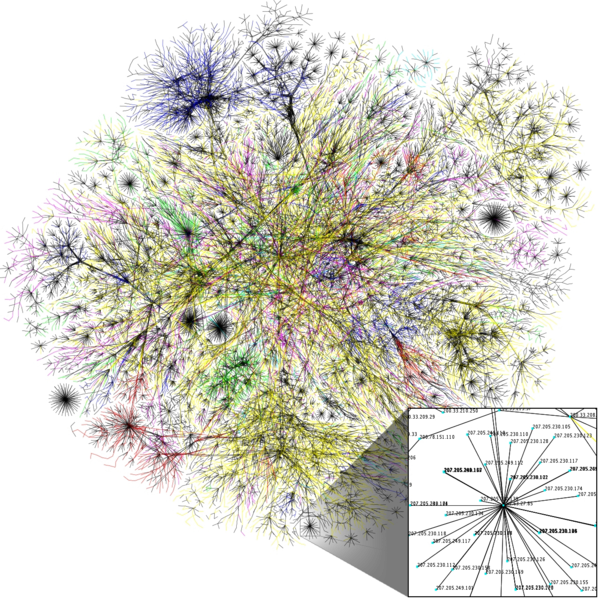
\includegraphics[width=\textwidth]{Internet_map}
	\label{fig:ill:internet}
\end{figure}

\subsection{Công nghệ web}

Công nghệ web là tổng hợp các công nghệ kỹ thuật phát triển web chạy trên môi trường máy chủ (mục \ref{subsection:webserver}) và trình duyệt web (mục \ref{subsection:webclient})

\paragraph{Máy chủ web \cite{web:server:what}} lưu trữ và cung cấp nội dung của một trang web - chẳng hạn như văn bản, hình ảnh, video và dữ liệu ứng dụng - cho khách hàng yêu cầu. Loại ứng dụng khách phổ biến nhất là chương trình trình duyệt web, trình duyệt yêu cầu dữ liệu từ trang web của bạn khi người dùng nhấp vào liên kết hoặc tải xuống tài liệu trên trang được hiển thị trong trình duyệt.

Máy chủ web giao tiếp với trình duyệt web bằng Giao thức truyền siêu văn bản (\acrshort{http}). Nội dung của hầu hết các trang web được mã hóa bằng Ngôn ngữ đánh dấu siêu văn bản (\acrshort{html}). Nội dung có thể tĩnh (ví dụ: văn bản và hình ảnh) hoặc động (ví dụ: giá đã tính hoặc danh sách các mặt hàng mà khách hàng đã đánh dấu để mua). Để cung cấp nội dung động, hầu hết các máy chủ web hỗ trợ ngôn ngữ kịch bản phía máy chủ để mã hóa logic nghiệp vụ vào giao tiếp. Các ngôn ngữ được hỗ trợ phổ biến bao gồm Active Server Pages (ASP), Javascript, PHP, Python và Ruby.

Máy chủ web cũng có thể lưu nội dung vào bộ nhớ cache để tăng tốc độ phân phối nội dung thường được yêu cầu. Quá trình này còn được gọi là tăng tốc web.

Máy chủ web có thể lưu trữ một trang web hoặc nhiều trang web sử dụng cùng một tài nguyên phần mềm và phần cứng, được gọi là lưu trữ ảo. Máy chủ web cũng có thể giới hạn tốc độ phản hồi đối với các máy khách khác nhau để ngăn một máy khách thống trị các tài nguyên được sử dụng tốt hơn để đáp ứng các yêu cầu từ một số lượng lớn máy khách.

Mặc dù máy chủ web thường lưu trữ các trang web có thể truy cập được trên Internet, chúng cũng có thể được sử dụng để giao tiếp giữa máy khách web và máy chủ trong các mạng cục bộ chẳng hạn như mạng nội bộ của công ty. Một máy chủ web thậm chí có thể được nhúng vào một thiết bị như một máy ảnh kỹ thuật số để người dùng có thể giao tiếp với thiết bị thông qua bất kỳ trình duyệt Web thông dụng nào.

\paragraph{\acrfull{html}} là một trong những thành phần cơ bản nhất để dựng thành web. Nó định nghĩa và cấu trúc nội dung của web.

"Siêu văn bản" đề cập đến các liên kết kết nối các trang web với nhau, trong một trang web hoặc giữa các trang web. Liên kết là một phần cơ bản của Web. Bằng cách tải nội dung lên Internet và liên kết nội dung đó với các trang do người khác tạo, bạn đã trở thành người tham gia trong World Wide Web.

\paragraph{\acrfull{css}} là một ngôn ngữ định kiểu sử dụng để mô tả các hiển thị của ngôn ngữ đánh dấu như \acrshort{html} và các ngôn ngữ tương tự. {\acrshort{css} mô tả cách mà các thành phần sẽ được hiển thị trên màn hình, trên giấy, khi nói và trên các phương tiện khác. {\acrshort{css} là một trong những ngôn ngữ chính của web mở và cũng là tiêu chuẩn trên các trình duyệt theo thông số W3C. Trước đây, việc phát triển các phần khác nhau của đặc tả CSS đã được thống nhất, cho phép tạo phiên bản cho các đề xuất mới nhất. Bạn có thể đã nghe nói về CSS1, CSS2.1, CSS3. Tuy nhiên, CSS4 chưa bao giờ trở thành phiên bản chính thức.

\subsection{Phân tích và thiết kế hệ thống}

\acrfull{uml} là một mô hình trực quan hóa nhằm:
\begin{itemize}
	\item Mô hình hóa nghiệp vụ và các tiến trình tương tự.
	\item Phân tích, thiết kế, triển khai các hệ thống phần mềm.
\end{itemize}
\acrfull{uml} là một ngôn ngữ phổ biến cho việc phân tích nghiệp vụ, kiến trúc phần mềm. Lập trình viên sử dụng nó để mô tả, yêu cầu, thiết kế, viết tài liệu cho: nghiệp vụ có sẵn hoặc yêu cầu nghiệp vụ mới, cấu trúc và hành vi của các hệ thống phần mềm.

\acrshort{uml} có thể được áp dụng cho các lĩnh vực ứng dụng đa dạng (ví dụ: ngân hàng, tài chính, internet, hàng không vũ trụ, chăm sóc sức khỏe, v.v.) Nó có thể được sử dụng với tất cả các phương pháp phát triển phần mềm đối tượng và thành phần chính và cho các nền tảng triển khai khác nhau.

\acrshort{uml} là một phương pháp mô hình hóa phần mềm, chứ không phải là quy trình phát triển phần mềm.
\begin{itemize}
\item cung cấp hướng dẫn về thứ tự các hoạt động của nhóm
\item chỉ định những gì tạo tác nên được phát triển
\item chỉ đạo nhiệm vụ của các nhà phát triển cá nhân và toàn bộ nhóm
\item đưa ra các tiêu chí để giám sát và đo lường các sản phẩm và hoạt động của dự án.
\end{itemize}
\acrshort{uml} chủ động độc lập với quy trình và có thể được áp dụng trong mọi bối cảnh của các quy trình khác nhau. Tuy nhiên, nó vẫn phù hợp nhất cho các quy trình phát triển theo hướng nhanh chóng đưa dự án vào sử dụng, lặp đi lặp lại và tăng dần.

\paragraph{Khái niệm hướng đối tượng \cite{book:oop} } được xây dựng trên nền tảng của khái niệm lập trình có cấu trúc và sự trừu tượng hóa dữ liệu. Sự thay đổi căn bản ở chỗ, một chương trình hướng đối tượng được thiết kế xoay quanh dữ liệu mà chúng ta có thể làm việc trên đó, hơn là theo bản thân chức năng của chương trình. Điều này hoàn toàn tự nhiên một khi chúng ta hiểu rằng mục tiêu của chương trình là xử lý dữ liệu. Suy cho cùng, công việc mà máy tính thực hiện vẫn thường được gọi là xử lý dữ liệu. Dữ liệu và thao tác liên kết với nhau ở một mức cơ bản (còn có thể gọi là mức thấp), mỗi thứ đều đòi hỏi ở thứ kia có mục tiêu cụ thể, các chương trình hướng đối tượng làm tường minh mối quan hệ này. Lập trình hướng đối tượng (Object Oriented Programming - gọi tắt là OOP) hay chi tiết hơn là Lập trình định hướng đối tượng, chính là phương pháp lập trình lấy đối tượng làm nền tảng để xây dựng thuật giải, xây dựng chương trình. Thực chất đây không phải là một phương pháp mới mà là một cách nhìn mới trong việc lập trình. Để phân biệt, với phương pháp lập trình theo kiểu cấu trúc mà chúng ta quen thuộc trước đây, hay còn gọi là phương pháp lập trình hướng thủ tục (Procedure-Oriented Programming), người lập trình phân tích một nhiệm vụ lớn thành nhiều công việc nhỏ hơn, sau đó dần dần chi tiết, cụ thể hoá để được các vấn đề đơn giản, để tìm ra cách giải quyết vấn đề dưới dạng những thuật giải cụ thể rõ ràng qua đó dễ dàng minh hoạ bằng ngôn ngữ giải thuật (hay còn gọi các thuật giải này là các chương trình con). Cách thức phân tích và thiết kế như vậy chúng ta gọi là nguyên lý lập trình từ trên xuống (top-down), để thể hiện quá trình suy diễn từ cái chung cho đến cái cụ thể. Các chương trình con là những chức năng độc lập, sự ghép nối chúng lại với nhau cho chúng ta một hệ thống chương trình để giải quyết vấn đề đặt ra. Chính vì vậy, cách thức phân tích một hệ thống lấy chương trình con làm nền tảng, chương trình con đóng vai trò trung tâm của việc lập trình, được hiểu như phương pháp lập trình hướg về thủ tục. Tuy nhiên, khi phân tích để thiết kế một hệ thống không nhất thiết phải luôn luôn suy nghĩ theo hướng “làm thế nào để giải quyết công việc”, chúng ta có thể định hướng tư duy theo phong cách “với một số đối tượng đã có, phải làm gì để giải quyết được công việc đặt ra” hoặc phong phú hơn, “làm cái gì với một số đối tượng đã có đó”, từ đó cũng có thể giải quyết được những công việc cụ thể. Với phương pháp phân tích trong đó đối tượng đóng vai trò trung tâm của việc lập trình như vậy, người ta gọi là nguyên lý lập trình từ dưới lên (Bottom-up). Lập trình hướng đối tượng liên kết cấu trúc dữ liệu với các thao tác, theo cách mà tất cả thường nghĩ về thế giới quanh mình. Chúng ta thường gắn một số các hoạt động cụ thể với một loại hoạt động nào đó và đặt các giả thiết của mình trên các quan hệ đó. 

\subsection{Kiến trúc hướng dịch vụ}
Kiến trúc hướng dịch vụ là một khái niệm để chỉ các hệ thống có kiến trúc chia nhỏ ra thành các phần nhỏ và đủ để giải quyết một vấn đề một cách độc lập. Kiến trúc này ra đời một các tự nhiên khi các kỹ sư cố gắng làm cho các thành phần ít phụ thuộc vào nhau hơn và từng thành phần được cấu trúc chắc chắn, ổn định và hiệu suất cao. 

Đối với một hệ thống máy chủ lớn, một dự án được chia thành rất nhiều thành phần để giao cho từng đội nhóm phát triển. Các hệ thống này đa số giao tiếp với nhau thông qua giao thức \acrshort{http}.

Kiến trúc hướng dịch vụ ngày một được sử dụng rộng rãi là một điều tất nhiên khi mà nghiệp vụ của các hệ thống đương đại ngày một phức tạp. Đội ngũ phát triển hệ thống không chỉ dừng lại ở vài ngàn người mà trong đó, mỗi thành phần được phát triển dựa trên hàng trăm công nghệ đồ sộ trước đó. Làm cho độ phức tạp của dự án tăng lên quá mức kiểm soát của một người hoặc một nhóm người.

Kiến trúc hướng dịch vụ có thể xem như một chức năng của một khối đối tượng. Các đối tượng này khi xem như một khối, thì sẽ sinh ra các phương thức tương ứng. Cách thiết kế này có thể giúp cho dịch vụ được phát triển một cách rõ ràng và hiệu suất hơn.

Kiến trúc hướng dịch vụ cũng chỉ phù hợp với một số quy mô dự án. Sử dụng kiến trúc không đúng với quy mô sẽ làm giảm tiến độ phát triển. Ảnh hưởng đến chất lượng hệ thống và khả năng nâng cấp sau này.

Để đáp ứng cho nhu cầu phân tách, một số khái niệm, công nghệ, phương pháp được triển khai ứng dụng. Cần hiệu và sử dụng các phương pháp để đảm bảo khả năng bảo mật cho hệ thống.

\subsection{Hệ quản trị cơ sở dữ liệu}
\subsubsection{Cơ sở dữ liệu NoSQL (phi quan hệ) hoạt động như thế nào? \cite{web:nosql}}

Cơ sở dữ liệu NoSQL sử dụng nhiều mô hình dữ liệu để truy cập và quản lý dữ liệu. Các loại cơ sở dữ liệu này được tối ưu hóa dành riêng cho các ứng dụng yêu cầu mô hình dữ liệu linh hoạt có lượng dữ liệu lớn và độ trễ thấp, có thể đạt được bằng cách giảm bớt một số hạn chế về tính nhất quán của dữ liệu của các cơ sở dữ liệu khác.



\begin{itemize}
	\item Trong cơ sở dữ liệu quan hệ, hồ sơ về một cuốn sách thường được phân tách (hay còn gọi là "chuẩn hóa") và lưu trữ trong các bảng tách biệt nhau, còn mối quan hệ được quy định bằng các ràng buộc khóa ngoại và khóa chính. Trong ví dụ này, bảng Sách có các cột cho ISBN, Tên sách và Số phiên bản, bảng Tác giả có các cột cho ID tác giả và Tên tác giả và cuối cùng, bảng Tác giả–ISBN có các cột cho ID tác giả và ISBN. Mô hình quan hệ được thiết kế để cho phép các cơ sở dữ liệu này thực thi tính toàn vẹn tham chiếu giữa nhiều bảng trong cơ sở dữ liệu, được chuẩn hóa để giảm dư thừa và thường được tối ưu hóa cho mục đích lưu trữ.
	\item Trong cơ sở dữ liệu NoSQL, hồ sơ về một cuốn sách thường được lưu trữ dưới dạng văn bản JSON. Với từng quyển sách, mục, ISBN, Tên sách, Số phiên bản, Tên tác giả và ID tác giả được lưu trữ dưới dạng thuộc tính trong một văn bản duy nhất. Trong mô hình này, dữ liệu được tối ưu hóa cho việc phát triển trực quan và khả năng thay đổi quy mô theo chiều ngang.
\end{itemize}
\subsubsection{Vì sao bạn nên sử dụng cơ sở dữ liệu NoSQL?\cite{web:nosql}}
Cơ sở dữ liệu NoSQL là lựa chọn cực kỳ thích hợp cho nhiều ứng dụng hiện đại, ví dụ như di động, web và trò chơi đòi hỏi phải sử dụng cơ sở dữ liệu cực kỳ thiết thực, linh hoạt, có khả năng thay đổi quy mô và hiệu năng cao để đem đến cho người dùng trải nghiệm tuyệt vời.
\begin{itemize}
	\item \textbf{Cơ sở dữ liệu NoSQL}: là lựa chọn cực kỳ thích hợp cho nhiều ứng dụng hiện đại, ví dụ như di động, web và trò chơi đòi hỏi phải sử dụng cơ sở dữ liệu cực kỳ thiết thực, linh hoạt, có khả năng thay đổi quy mô và hiệu năng cao để đem đến cho người dùng trải nghiệm tuyệt vời.
	\item \textbf{Khả năng thay đổi quy mô}: Cơ sở dữ liệu NoSQL thường được thiết kế để tăng quy mô bằng cách sử dụng các cụm phần cứng được phân phối thay vì tăng quy mô bằng cách bổ sung máy chủ mạnh và tốn kém. Một số nhà cung cấp dịch vụ đám mây xử lý các hoạt động này một cách không công khai dưới dạng dịch vụ được quản lý đầy đủ.
	\item \textbf{Hiệu năng cao}: Cơ sở dữ liệu NoSQL được tối ưu hóa theo các mô hình dữ liệu cụ thể và các mẫu truy cập giúp tăng hiệu năng cao hơn so với việc cố gắng đạt được mức độ chức năng tương tự bằng cơ sở dữ liệu quan hệ.
	\item \textbf{Cực kỳ thiết thực}: Cơ sở dữ liệu NoSQL cung cấp các API và kiểu dữ liệu cực kỳ thiết thực được xây dựng riêng cho từng mô hình dữ liệu tương ứng.
\end{itemize}
\subsection{Quản lí mã nguồn}

Git là một hệ thống kiểm soát phiên bản phân tán. Một mã nguồn mở miễn phí được thiết kế để xử lý mọi thứ từ các dự án nhỏ đến rất lớn với tốc độ và hiệu quả.

Git rất dễ học và đặc biệt hiệu suất. Nó vượt trội hơn các công cụ SCM như Subversion, CVS, Perforce và ClearCase với các tính năng như tối ưu phân nhánh cục bộ, thực hiện đóng gói và nhiều quy trình làm việc.

\begin{figure}[h]
	\caption{Hệ thống kiểm soát phiên bản, nguồn: git-scm.com}
	\centering
	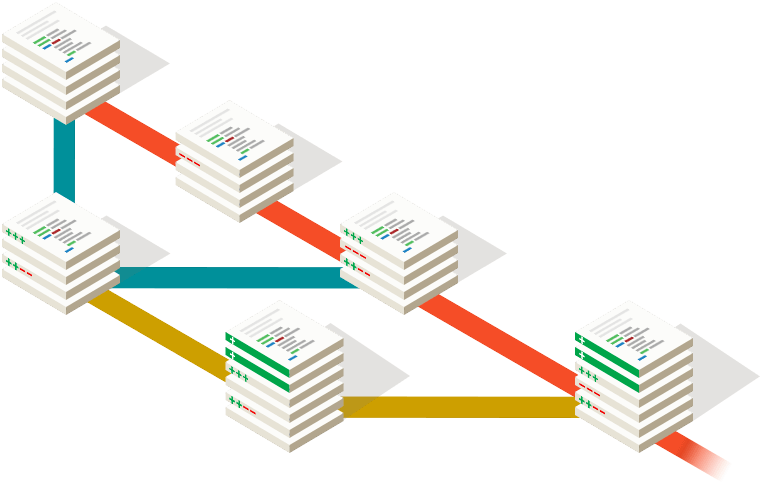
\includegraphics[width=\textwidth]{git}
	\label{fig:ill:git}
\end{figure}

\subsubsection{Phân nhánh và Hợp nhất}
Tính năng Git thực sự khác biệt với SCM là mô hình phân nhánh của nó.
Git cho phép và khuyến khích bạn có nhiều chi nhánh cục bộ có thể hoàn toàn độc lập với nhau. Việc tạo, hợp nhất và xóa các dòng phát triển đó mất vài giây.

\subsubsection{Nhỏ và nhanh}
Git rất nhanh. Với Git, gần như tất cả các hoạt động đều được thực hiện cục bộ, mang lại lợi thế về tốc độ rất lớn trên các hệ thống tập trung liên tục phải giao tiếp với máy chủ ở đâu đó.
Git được xây dựng để hoạt động trên nhân Linux, có nghĩa là nó phải xử lý hiệu quả các kho lưu trữ lớn ngay từ đầu. Git được viết bằng \acrshort{c}, giảm chi phí thời gian chạy liên quan đến các ngôn ngữ cấp cao hơn. Tốc độ và hiệu suất là mục tiêu thiết kế chính của Git ngay từ đầu.

\subsubsection{Được phân phối}
Một trong những tính năng hay nhất của bất kỳ hệ phân tán SCM nào, bao gồm Git, là nó được phân tán. Điều này có nghĩa là thay vì thực hiện "checkout" hiện tại của mã nguồn, bạn thực hiện "clone" toàn bộ kho lưu trữ.

\section{Công cụ}

\subsection{Node.js}
% {Font: Time New Roman; đậm; cỡ chữ: 13; dãn dòng: 1,3; căn{Font: Time New Roman; đậm; cỡ chữ: 13; dãn dòng: 1,3; căn lề: justified}
Là một môi trường chạy JavaScript theo hướng sự kiện bất đồng bộ, Node.js được thiết kế để xây dựng các ứng dụng mạng có thể mở rộng.

Một trong những lý do kiến Node.js trở nên phổ biến là nhờ sự phổ biến của Javascript. Tại thời điểm Javascript phát triển mạnh mẽ ở phía trình duyệt máy khách. Thì Node.js với hàng loạt các thư viện mạnh mẽ đã mang đến trải nghiệm phát triển liền mạch. Ngoài sự linh hoạt và quen thuộc đã nêu, hiệu suất của Node.js cũng khá tốt để phát triển một hệ thống máy chủ dẻo dai hơn.

\subsection{PM2.js}
Để phát hành ứng dụng máy chủ web lên một máy chủ ảo. Cần khởi chạy pm2 như một phần mềm quản lí tiến trình.
pm2 giúp ta có thể khởi động lại, xóa hoặc chạy các tiến trình khi mà phiên kết nối giữa máy chủ và máy khách bị đóng.

Thay thế pm2, có thể sử dụng thư viện có sẵn của Node.js để lưu trữ mã tiến trình và khởi động hoặc xóa nó khi cần. Nhưng điều này tốn thời gian và độ hoàn thiện không đủ để thay thế pm2 khi nó còn là một mã nguồn mở miễn phí.

Khi thực hiện triển khai một hệ thống hướng dịch vụ với hàng trăm tiến trình. Nhu cầu kiểm tra theo dõi tình trạng các tiến trình tại một đầu mối tổng là hết sức cần thiết. PM2 cũng cung cấp gói tính phí để giải quyết vấn đề này. Tuy nhiên, so với các dịch vụ quản lí tiến trình khác thì cần phải cân nhắc.

Phát triển một hệ thống quản lí tiến trình tập trung cần hiểu các kiến thức về hệ thống phân tán. Điều này cũng không đơn giản khi các tiến trình hoặc các máy chủ ảo liên tục bị quá tải và khởi động lại. Lúc này các phương án dự phòng và khôi phục cần được thiết đặt và sử dụng.

\subsection{React.js \cite{web:react}} 
Một thư viện JavaScript xây dựng giao diện người dùng

\subsubsection{Tính trực quan}
% {Font: Time New Roman; đậm & nghiêng; cỡ chữ: 13; dãn dòng: 1,3; căn lề: justified}
React giúp tạo các UI tương tác một cách dễ dàng. Thiết kế các khung nhìn đơn giản cho từng trạng thái trong ứng dụng của bạn, và React sẽ cập nhật và kết xuất đúng các thành phần phù hợp khi dữ liệu thay đổi.

Việc khai báo các khung nhìn tường minh sẽ khiến cho mã của bạn dễ sử dụng hơn và dễ dàng gỡ lỗi hơn.

\subsubsection{Dựa trên khối cơ bản}
Xây dựng các khối cơ bản và quản lý các trạng thái của riêng chúng, sau đó kết hợp chúng để tạo các giao diện người dùng phức tạp.

Vì khối cơ bản được viết bằng JavaScript thay vì các mẫu, bạn có thể dễ dàng truyền dữ liệu đa dạng qua ứng dụng của mình và tránh thao tác với DOM.

\subsubsection{Dễ học, dễ làm}
React không đưa ra các giả định về phần kĩ năng công nghệ của bạn, vì vậy bạn có thể phát triển các tính năng mới trong React mà không cần viết lại mã hiện có.

React cũng có thể kết xuất trên máy chủ bằng Node và xây dựng ứng dụng di động bằng cách sử dụng React Native.

\subsection{Next.js}
Next.js là một sự kết hợp giữa việc kết xuất khối cơ bản của React.js ở môi trường trình duyệt với môi trường máy chủ một cách linh hoạt.
Next.js là một máy chủ Node.js sử dụng React.js nên cung cấp khả năng điều hướng. Đọc dữ liệu và truyền tải dữ liệu giữa hai môi trường một cách hết sức linh hoạt và mạnh mẽ.
Một khối cơ sở của React.js được viết ra trong Next.js liền mạch đến mức nếu lập trình viên không nắm rõ kiến thức nền tảng và hiểu về Next.js sẽ không kiểm soát được rằng rốt cuộc dòng lệnh đó được thực thi và kết xuất ở máy chủ hay trình duyệt máy khách.
Các phiên bản sau này của Next.js ra đời hạn chế sự liền mạch giữa hai môi trường để giảm bớt sự nhập nhằng cho lập trình viên.
Next.js thực sự mạnh mẽ nhưng cũng không phải là lựa chọn duy nhất. Có rất nhiều thư viện tương tự ra đời và còn hiệu quả hơn cả Next.js.

Next.js cung cấp đầy đủ các khả năng để tạo ra một khối máy chủ web hoàn chỉnh. Nhưng đa số người dùng sử dụng nó như một dịch vụ kết xuất giao diện trong hệ thống kiến trúc hướng dịch vụ của họ.

Bởi khả năng kết xuất, điều hướng và truyền tải dữ liệu giữa hai môi trường linh hoạt. Trải nghiệm người dùng ở trình duyệt được cải thiện rõ rệt. Những vấn đề về tối ưu, cập nhật thông tin, gọi dữ liệu kết xuất phức tạp được giải quyết dễ dàng hơn.

\subsection{GraphQL}

\subsubsection{REST API \cite{web:rest}}

\begin{figure}[h]
	\caption{REST API}
	\centering
	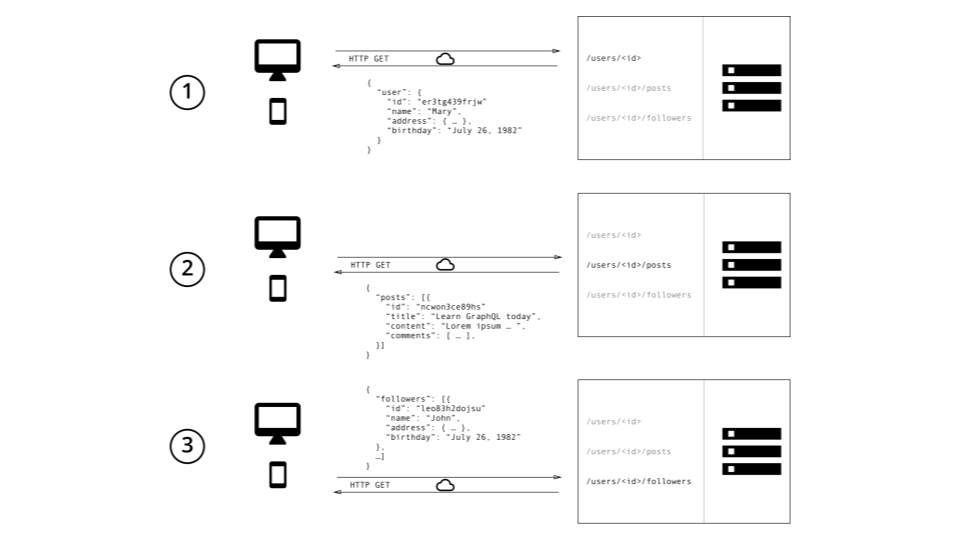
\includegraphics[width=\textwidth]{rest}
	\label{fig:ill:rest}
\end{figure}
REST là gì?
Chuyển trạng thái đại diện (REST) là một kiến trúc phần mềm quy định các điều kiện về cách thức hoạt động của API. REST ban đầu được tạo ra như một hướng dẫn để quản lý giao tiếp trên một mạng phức tạp như Internet. Bạn có thể sử dụng kiến trúc dựa trên REST để hỗ trợ giao tiếp hiệu suất cao và đáng tin cậy trên quy mô lớn. Bạn có thể dễ dàng triển khai và sửa đổi REST, mang lại khả năng hiển thị và tính di động đa nền tảng cho bất kỳ hệ thống API nào.


\subsubsection{GraphQL API}

GraphQL là ngôn ngữ truy vấn cho các API và thời gian thực để thực hiện các truy vấn đó với dữ liệu hiện có của bạn. GraphQL cung cấp mô tả đầy đủ và dễ hiểu về dữ liệu trong API, cung cấp cho khách hàng sức mạnh để yêu cầu chính xác những gì họ cần và không cần gì hơn, giúp việc phát triển API dễ dàng hơn theo thời gian và cho phép các công cụ mạnh mẽ dành cho nhà phát triển.

\begin{figure}[h]
	\caption{GraphQL API}
	\centering
	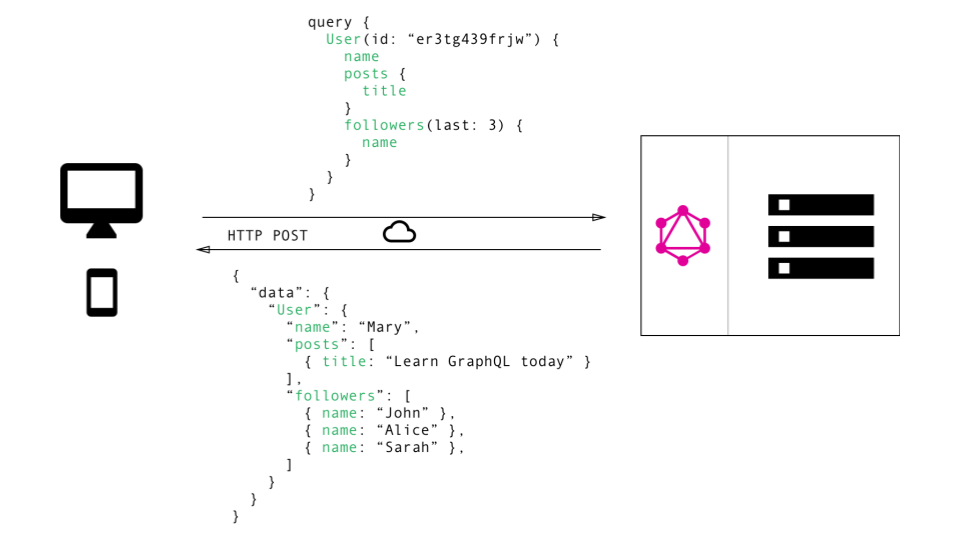
\includegraphics[width=\textwidth]{graph}
	\label{fig:ill:graph}
\end{figure}

\pagebreak

\subsection{Apollo Server}
Nhờ sức mạnh của ngôn ngữ truy vấn dành cho API là GraphQL. Apollo Server thiết kế ra để dễ dàng khởi tạo khung sườn cho dự án sử dụng GraphQL để phân tích cú pháp và xử lí nghiệp vụ dễ dàng hơn.

Khác với REST API và cấu trúc MVC thông thường. GraphQL tổ chức xử lí API theo kiểu quy nạp. Cú pháp được phân tích thành cấu trúc cây và chia ra xử lí sau đó quy nạp ngược lên để trả kết quả về phía người dùng.

GraphQL cũng cho phép định kiểu các chức năng xử lí và hoạt động truy cập đến đối tượng nên có thể chia cấu trúc dự án hướng đối tượng với các hàm xử lí rất nhỏ. Mỗi hàm chức năng như vậy đều có thể là một nút trên cây truy vấn. Điều này giúp cho việc truy vấn và khởi chạy các hàm, liên kết quy nạp dữ liệu diễn ra hết sức linh hoạt. Nghĩa là bạn có thể lấy duy nhất một bảng ghi sau đó xử lí. Hoặc lấy danh sách bản ghi bao gồm việc xử lí đều được mà không cần phát triển một "Controller" mới như mô hình MVC thông thường.

\begin{figure}
	\centering
	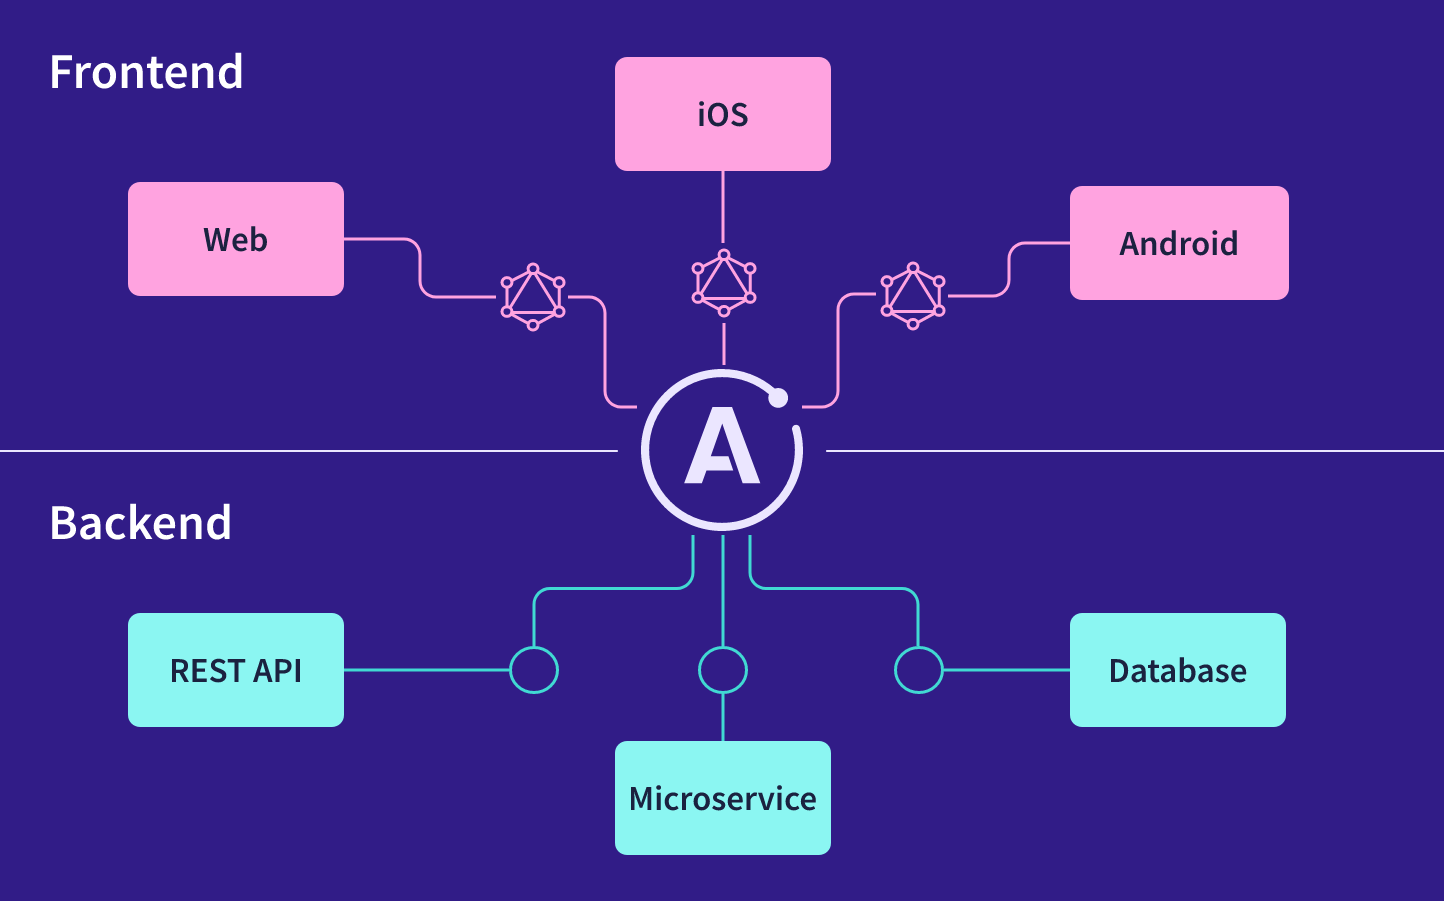
\includegraphics[width=0.7\linewidth]{images/apollo-server}
	\caption[Kiến trúc Apollo Server]{}
	\label{fig:apollo-server}
\end{figure}

Một số người nhờ vào sự linh hoạt khi thiết kế các nút xử lí của GraphQL để xử dụng chúng như một Gateway cho hệ thống có sẵn của họ. Tạo nên một bộ API thống nhất trên một tài liệu lập trình duy nhất giúp cho các đội ngũ có thể giao tiếp với nhau dễ dàng hơn và tài liệu được cập nhật triệt để hơn.

\subsection{MongoDB}
MongoDB là một mã nguồn mở để quản lí cơ sở dữ liệu dạng tài liệu thay vì dạng bảng như \acrshort{sql}. MongoDB được phát triển để mở rộng theo chiều ngang làm cho định kiểu dữ liệu trở nên linh hoạt hơn. Phát hành năm 2007, MongoDB đã được tiếp nhận và phổ biến khắp nơi trên thế giới.

Thay vì lưu dữ liệu vào bảng theo hàng hoặc cột như \acrshort{sql}, mỗi bản ghi trong MongoDB được mô tả như một tài liệu BJSON, dạng mã hóa nhị phân dữ liệu. Ứng dụng có thể duyệt qua những thông tin theo định dạng JSON.

Lưu trữ database dạng tài liệu như vậy rất linh hoạt, chúng cho phép tùy biến trong cấu trúc của mỗi tài liệu và chỉ lưu một phần của tài liệu. Một tài liệu có thể có các dạng dữ liệu khác nhau. Từng trường dữ liệu cũng có khả năng ràng buộc giá trị như một cột của \acrshort{sql}.Ta cũng có thể đánh indexed để gia tăng tốc độ truy vấn.

No-SQL với những ưu điểm của nó rất thích hợp khi dùng để phát triển một dự chưa rõ ràng. Với một dự án quá lớn. Không nên chỉ sử dụng một loại quản trị cơ sở dữ liệu. Từng trường hợp cụ thể. Với kiến thức về ưu nhược điểm của từng loại ta nên lựa chọn phương án phù hợp hơn là so sách mà bỏ các vấn đề giải quyết ngay trong dự án hiện tại.
\section{Dịch vụ}
Luận án sử dụng một số dịch vụ của bên thứ ba để lược bớt sự phức tạp và khối lượng của dự án. Các vấn đề này xử lí rất đơn giản khi sử dụng dịch vụ bên ngoài. Sự phụ thuộc là không đáng kể. Cần đưa ra các phương án dự phòng khi phát triển. Cần phát triển các cầu nối đủ linh hoạt để sử dụng nhiều dịch vụ và lựa chọn giữa các nhà cung cấp trở nên dễ dàng hơn.

\subsection{Dịch vụ lưu trữ}
Dịch vụ lưu trữ được sử dụng tại luận án là dịch vụ lưu trữ tài nguyên đơn giản nhất. Chỉ có chức năng đăng tải và truy cập. Không hỗ trợ tìm kiếm, nén tệp, tối ưu hình ảnh.

\subsection{Dịch vụ địa chỉ}
Dịch vụ địa chỉ cung cấp danh sách tỉnh thành, quận huyện và các thông tin địa danh cấp nhỏ hơn để khách hàng khai báo thông tin địa chỉ. Các dịch vụ cung cấp thông tin đầy đủ, chính xác và được cập nhật thường xuyên.

\subsection{Dịch vụ thư điện tử}
Dịch vụ thư điên tử sử dụng là máy chủ thư điện tử. Việc cấu hình máy chủ thư điện tử và chi phí duy trì một máy chủ độc lập là không cần thiết.

Các nhà cung cấp dịch vụ thư điện tử cũng cung cấp giao diện người dùng đầy đủ tính năng giúp duyệt thư dễ dàng hơn.

\subsection{Dịch vụ tên miền}
Dịch vụ máy chủ tên miền giúp phân giải tên miền đến một địa chỉ ip cụ thể. Máy chủ tên miền sử dụng không bao gồm chứng thực SSL và cân bằng tải.

Máy chủ tên miền \cite{web:dns} chứa thông tin lưu trữ về một số tên miền. Hệ thống phân giải tên miền được vận hành bởi hệ thống dữ liệu phân tán, dạng Client-Server. Các node của hệ thống dữ liệu này là các máy chủ tên miền. Mỗi một tên miền sẽ có ít nhất một máy chủ tên miền chứa thông tin về tên miền đó. Các thông tin về máy chủ tên miền sẽ được lưu trữ trong các zone của tên miền. Có hai dạng Name Server là là Primary và Secondary. Một Client sẽ ưu tiên hỏi Primary trước và thử lại với Secondary nếu Primary không thể trả lời thông tin về tên miền đó trong thời gian quy định.

\subsection{Dịch vụ máy chủ ảo}
Đề tài không bao gồm việc cấu hình mạng, phần cứng của máy chủ. Để triển khai mã nguồn dự án lên môi trường thực tế. Đề tài mô tả việc cấu hình mã nguồn dự án lên một máy chủ ảo (định nghĩa máy chủ mục \ref{subsection:webserver}).